\documentclass[12pt, a4paper]{report}

\usepackage[a4paper,width=150mm,top=25mm,bottom=25mm,bindingoffset=6mm]{geometry}
%\usepackage[compact]{titlesec}
\usepackage[T1]{fontenc} 								
\usepackage[norsk]{babel}								
\usepackage[utf8]{inputenc}						
\usepackage{graphicx}       						
%\usepackage{amsmath,amssymb}
%\usepackage{grffile}
%\usepackage{listings}
%\usepackage{caption}
%\usepackage[export]{adjustbox}
\usepackage{titling}
\setcounter{secnumdepth}{0}

%\lstset{extendedchars=true, basicstyle=\footnotesize, numbers=left, numberstyle=\tiny, frame=shadowbox, tabsize=2, language=C, showstringspaces=false, breaklines=true,
%  literate=
  %{á}{{\'a}}1 {é}{{\'e}}1 {í}{{\'i}}1 {ó}{{\'o}}1 {ú}{{\'u}}1
  %{Á}{{\'A}}1 {É}{{\'E}}1 {Í}{{\'I}}1 {Ó}{{\'O}}1 {Ú}{{\'U}}1
  %{à}{{\`a}}1 {è}{{\`e}}1 {ì}{{\`i}}1 {ò}{{\`o}}1 {ù}{{\`u}}1
 % {À}{{\`A}}1 {È}{{\'E}}1 {Ì}{{\`I}}1 {Ò}{{\`O}}1 {Ù}{{\`U}}1
  %{ä}{{\"a}}1 {ë}{{\"e}}1 {ï}{{\"i}}1 {ö}{{\"o}}1 {ü}{{\"u}}1
  %{Ä}{{\"A}}1 {Ë}{{\"E}}1 {Ï}{{\"I}}1 {Ö}{{\"O}}1 {Ü}{{\"U}}1
  %{â}{{\^a}}1 {ê}{{\^e}}1 {î}{{\^i}}1 {ô}{{\^o}}1 {û}{{\^u}}1
  %{Â}{{\^A}}1 {Ê}{{\^E}}1 {Î}{{\^I}}1 {Ô}{{\^O}}1 {Û}{{\^U}}1
  %{ã}{{\~a}}1 {Ã}{{\~A}}1 {õ}{{\~o}}1 {Õ}{{\~O}}1
  %{œ}{{\oe}}1 {Œ}{{\OE}}1 {æ}{{\ae}}1 {Æ}{{\AE}}1 {ß}{{\ss}}1
  %{ç}{{\c c}}1 {Ç}{{\c C}}1 {ø}{{\o}}1 {å}{{\r a}}1 {Å}{{\r A}}1
  %{€}{{\EUR}}1 {£}{{\pounds}}1}

\setlength{\textheight}{240mm} 
\setlength{\textwidth}{180mm}  
\topmargin -5mm 
\oddsidemargin -5mm

\pretitle{%
  \begin{center}
  \LARGE
  
\includegraphics[width=6cm,height=6cm]{uitlogo.png}
}
\posttitle{\end{center}}

\begin{document}
\title{\\Praksis hos Norut}
%\titlespacing*{\chapter}{0pt}{-70mm}{40pt}
\author{Fredrik Sandhei\thanks{UiT - TEK-2000, obligatorisk rapport.}}

\date{\today}
\maketitle
\newpage
\tableofcontents
\newpage

\section{Introduksjon}
TEK-2000 ''Praksis som valgemne'' er et av de tre emnene jeg har valgt for 5.semesteret mitt på 3.året i droneteknologi. Emnet går ut på at studenten skal ha en praksis hos en bedrift som er passende til utdannelsen. Praksisplassen må fylle kriterier fra emneansvarlig på bedriftens relevans til utdannelsen. \\
Jeg søkte praksis hos to plasser, Luftfartstilsynet og Norut. Begge er relevante på hver sin måte. Jeg fikk innpass hos begge, men på grunn av lokalitet og mest relevanse valgte jeg Norut. Rune Storvold er forskningssjef hos Norut og er ansvarlig for min praksisperiode i Norut. Praksisen foregår i 20 dager. Jeg avtalte med Rune Storvold at praksisen skulle gjennomføres i et kontinuerlig kjør. Praksisen begynte i uke 33 og avsluttet i uke 37. En arbeidsdag hos Norut går fra 08:00 - 15:00. Etter endt praksis skulle en rapport leveres inn fra studenten om praksisperioden. 
%FÅ RETNINGSLINJENE FOR RAPPORTEN...
%Beskriv emnet, hensikten og hva som må gjøres
%FÅ MAL FRA EMNEANSVARLIG

\newpage
\section{Hendelsesforløp}
%Kort om hver uke. Få frem meningen med alt
%Få beskrevet arbeidsoppgavene, forhåpentligvis ei liste 
%som blir oversiktlig.
%Litt frem og tilbake på hva jeg driver med
\subsection{Uke 1 og prosjekt}
\subsubsection{Backlog og GIS}
%Back log av flight plans
%Flyoperativ avdeling 
%Avdelingsmøte
Den første dagen begynte med introduksjon av meg til personalet og bli kjent med lokale. Deretter ble jeg satt rett i arbeid med backlog av tidligere flight plan inn i det GIS-baserte loggsystemet. \\
Typisk metodikk innen luftfart (fra erfaringsmessig område) er ''learning by doing''. Poenget er for best læringskapasitet med å bare ''prøve ut'' litt for seg selv, og ta utgangspunkt i eksempler som er gitt.\\
En flight log er et skjema som beskriver en flyoperasjon. I denne loggen skal det minimum være flytype, tidspunkt for take-off, landing, tid i lufta, drivstoff brukt, hvilke luftfartsinstans man har vært i kontakt med om noe, vær og så videre. %kom med beskrivelse...

%Bilde av loggskjema
\begin{figure}[h]
	\centering
	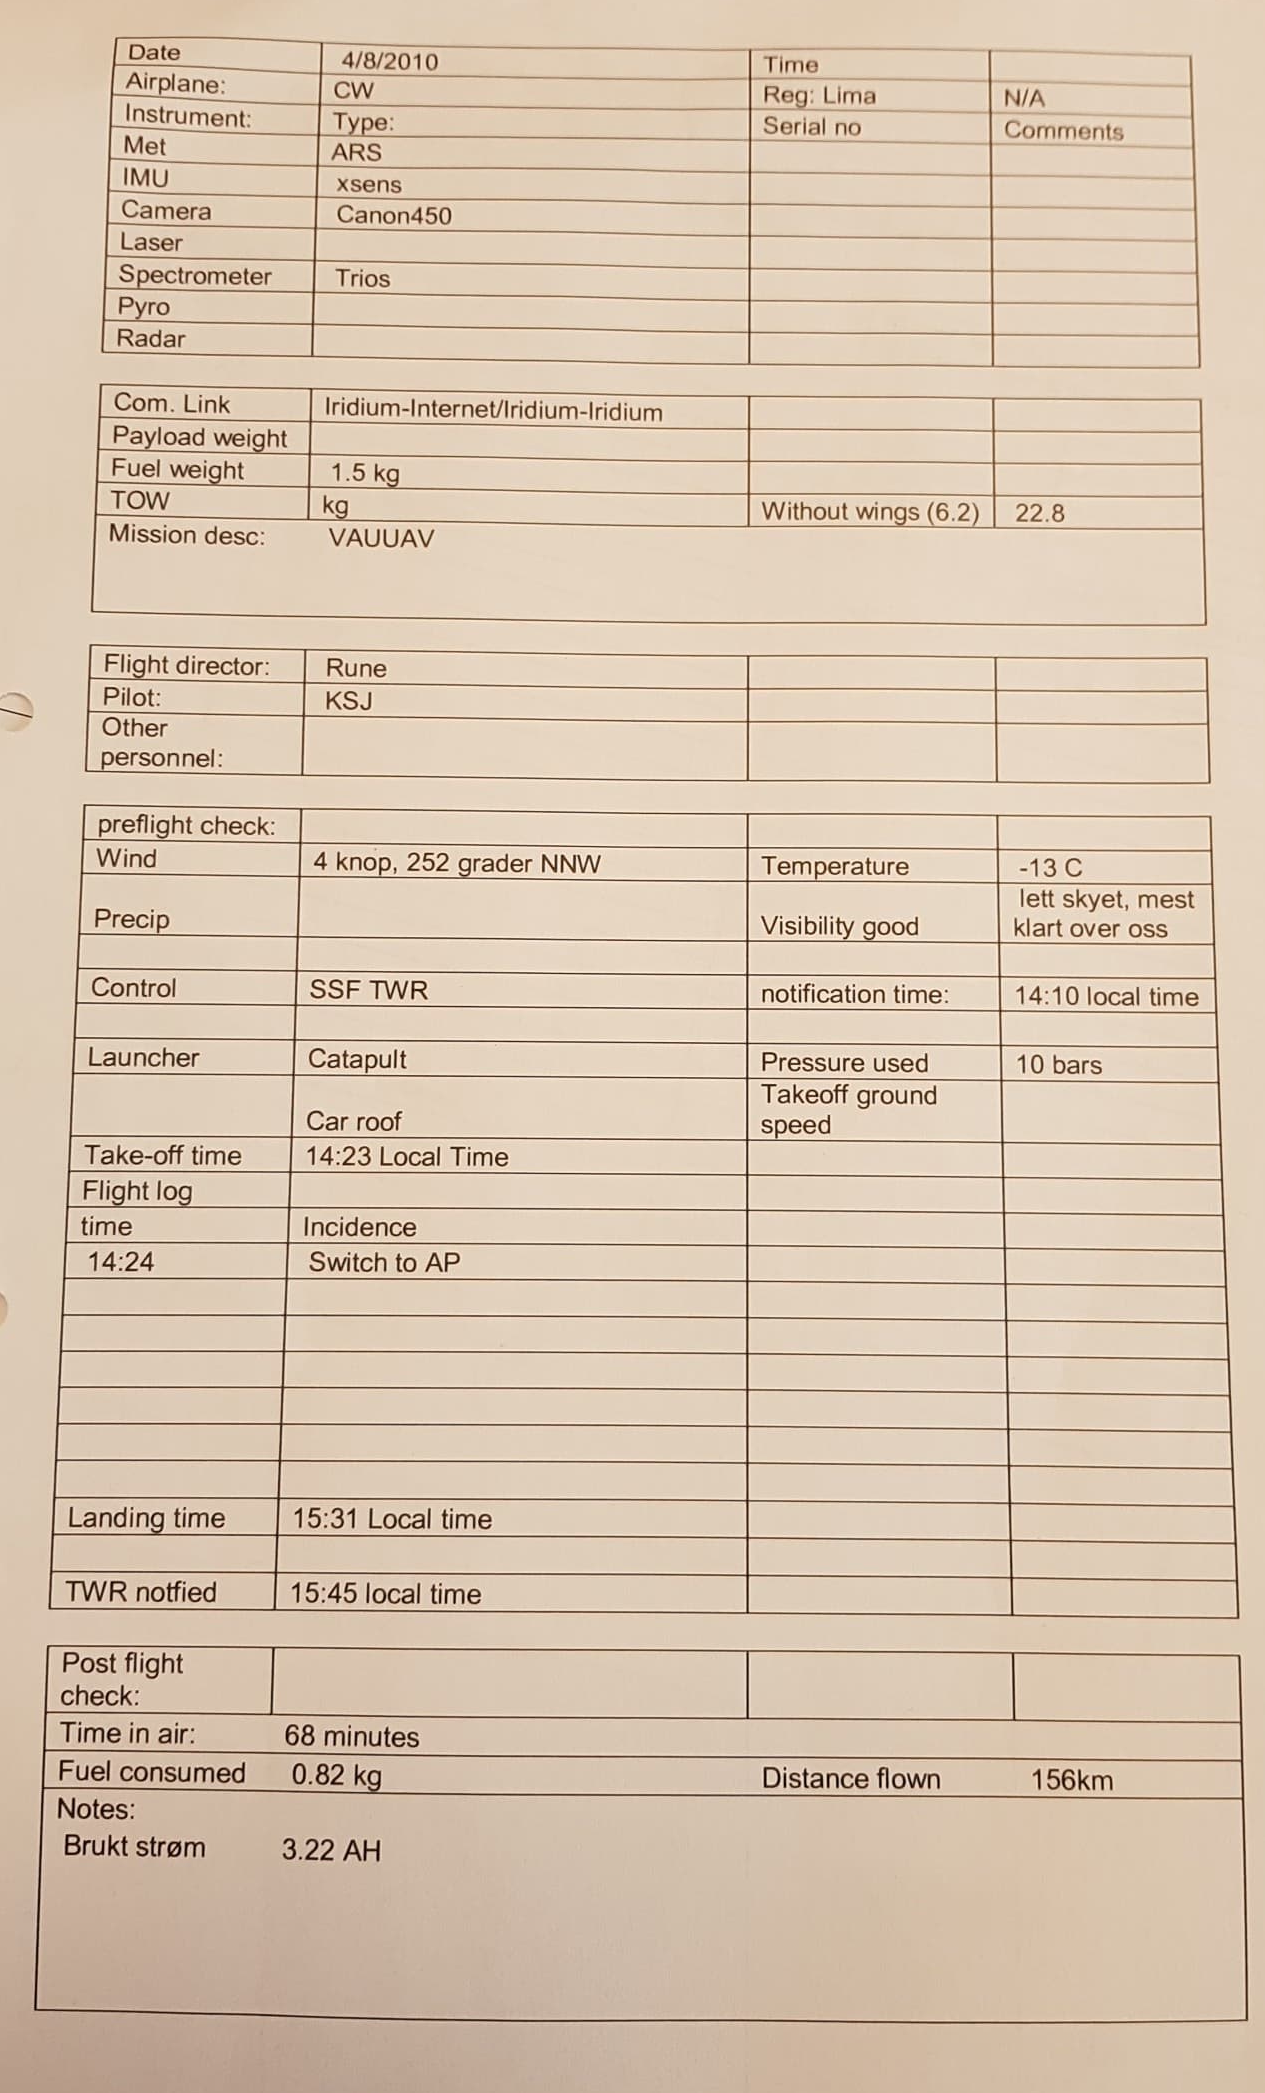
\includegraphics[height= 10cm, width=0.5\textwidth]{flightlogNorut.png}
		\caption{Typisk opplegg av loggskjema til Norut. Skjemaet skal inneholde nødvendig informasjon om flighten som kan brukes til gjennomgang for neste flight. }
\end{figure}
\newpage
Mesteparten av den første dagen gikk til backlog samt et avdelingsmøte som jeg fikk muligheten til å delta på.\\
\subsubsection{Byggeprosjekt}
Dag 2 fikk jeg et prosjekt utdelt som jeg skulle fokusere med i de neste ukene. Prosjektet gikk ut på bygging og testflyvning av tre fly av typen Cryowing Observer. \\
Flyene skulle også dokumenteres luftdyktigheten på, det vil si at det må dokumenteres i hvor god stand disse er til å følge kravene satt av Norut for sikker flyvning. Til forberedelse av prosjektet ble jeg bedt om å legge opp en plan for hvordan jeg vil finne de ulike egenskapene til flyene, som skal dokumenteres i en såkalt POH (Pilot's Operating Handbook). I denne POH'en skulle jeg blant annet finne følgende opplysninger gjennom testflygninger: 
\begin{itemize}
	\item Cruise speed
	\item Stall speed
	\begin{itemize}
		\item Flap up power off
		\item Half flap power off
		\item Full flap power off	
	\end{itemize}
	\item Standard empty weight
	\item Maximal Take Off Weight (MTOW)
	\item Wing loading
	\item Power loading
\end{itemize}
Oppsettet jeg lagde for testflygningen er vedlagt i appendix-biten av rapporten, se innholdsfortegnelsen. \\
Selve byggingen av luftfartøyene kunne ikke begynne før uke 2, da delene måtte hentes opp fra Bodø. \\ 
\newpage
I mellomtiden drev jeg med reparasjonsarbeid på et av Noruts multirotorer som havarerte. Nye rammer måtte settes på, elektroniske fartskontrollere måtte kobles opp og konfigureres og mer. Da jeg har drevet med noe bygging av multirotorer i hobbybasis, samt fått teoretisk kompetanse fra emnene på studiet, gikk mye av arbeidet bra. Konfigurasjonene som Norut bruker (se bildene under), var litt nytt, men prinsippet var det samme som på hobbyprosjektene mine. \\

\begin{figure}[h]
	\centering
	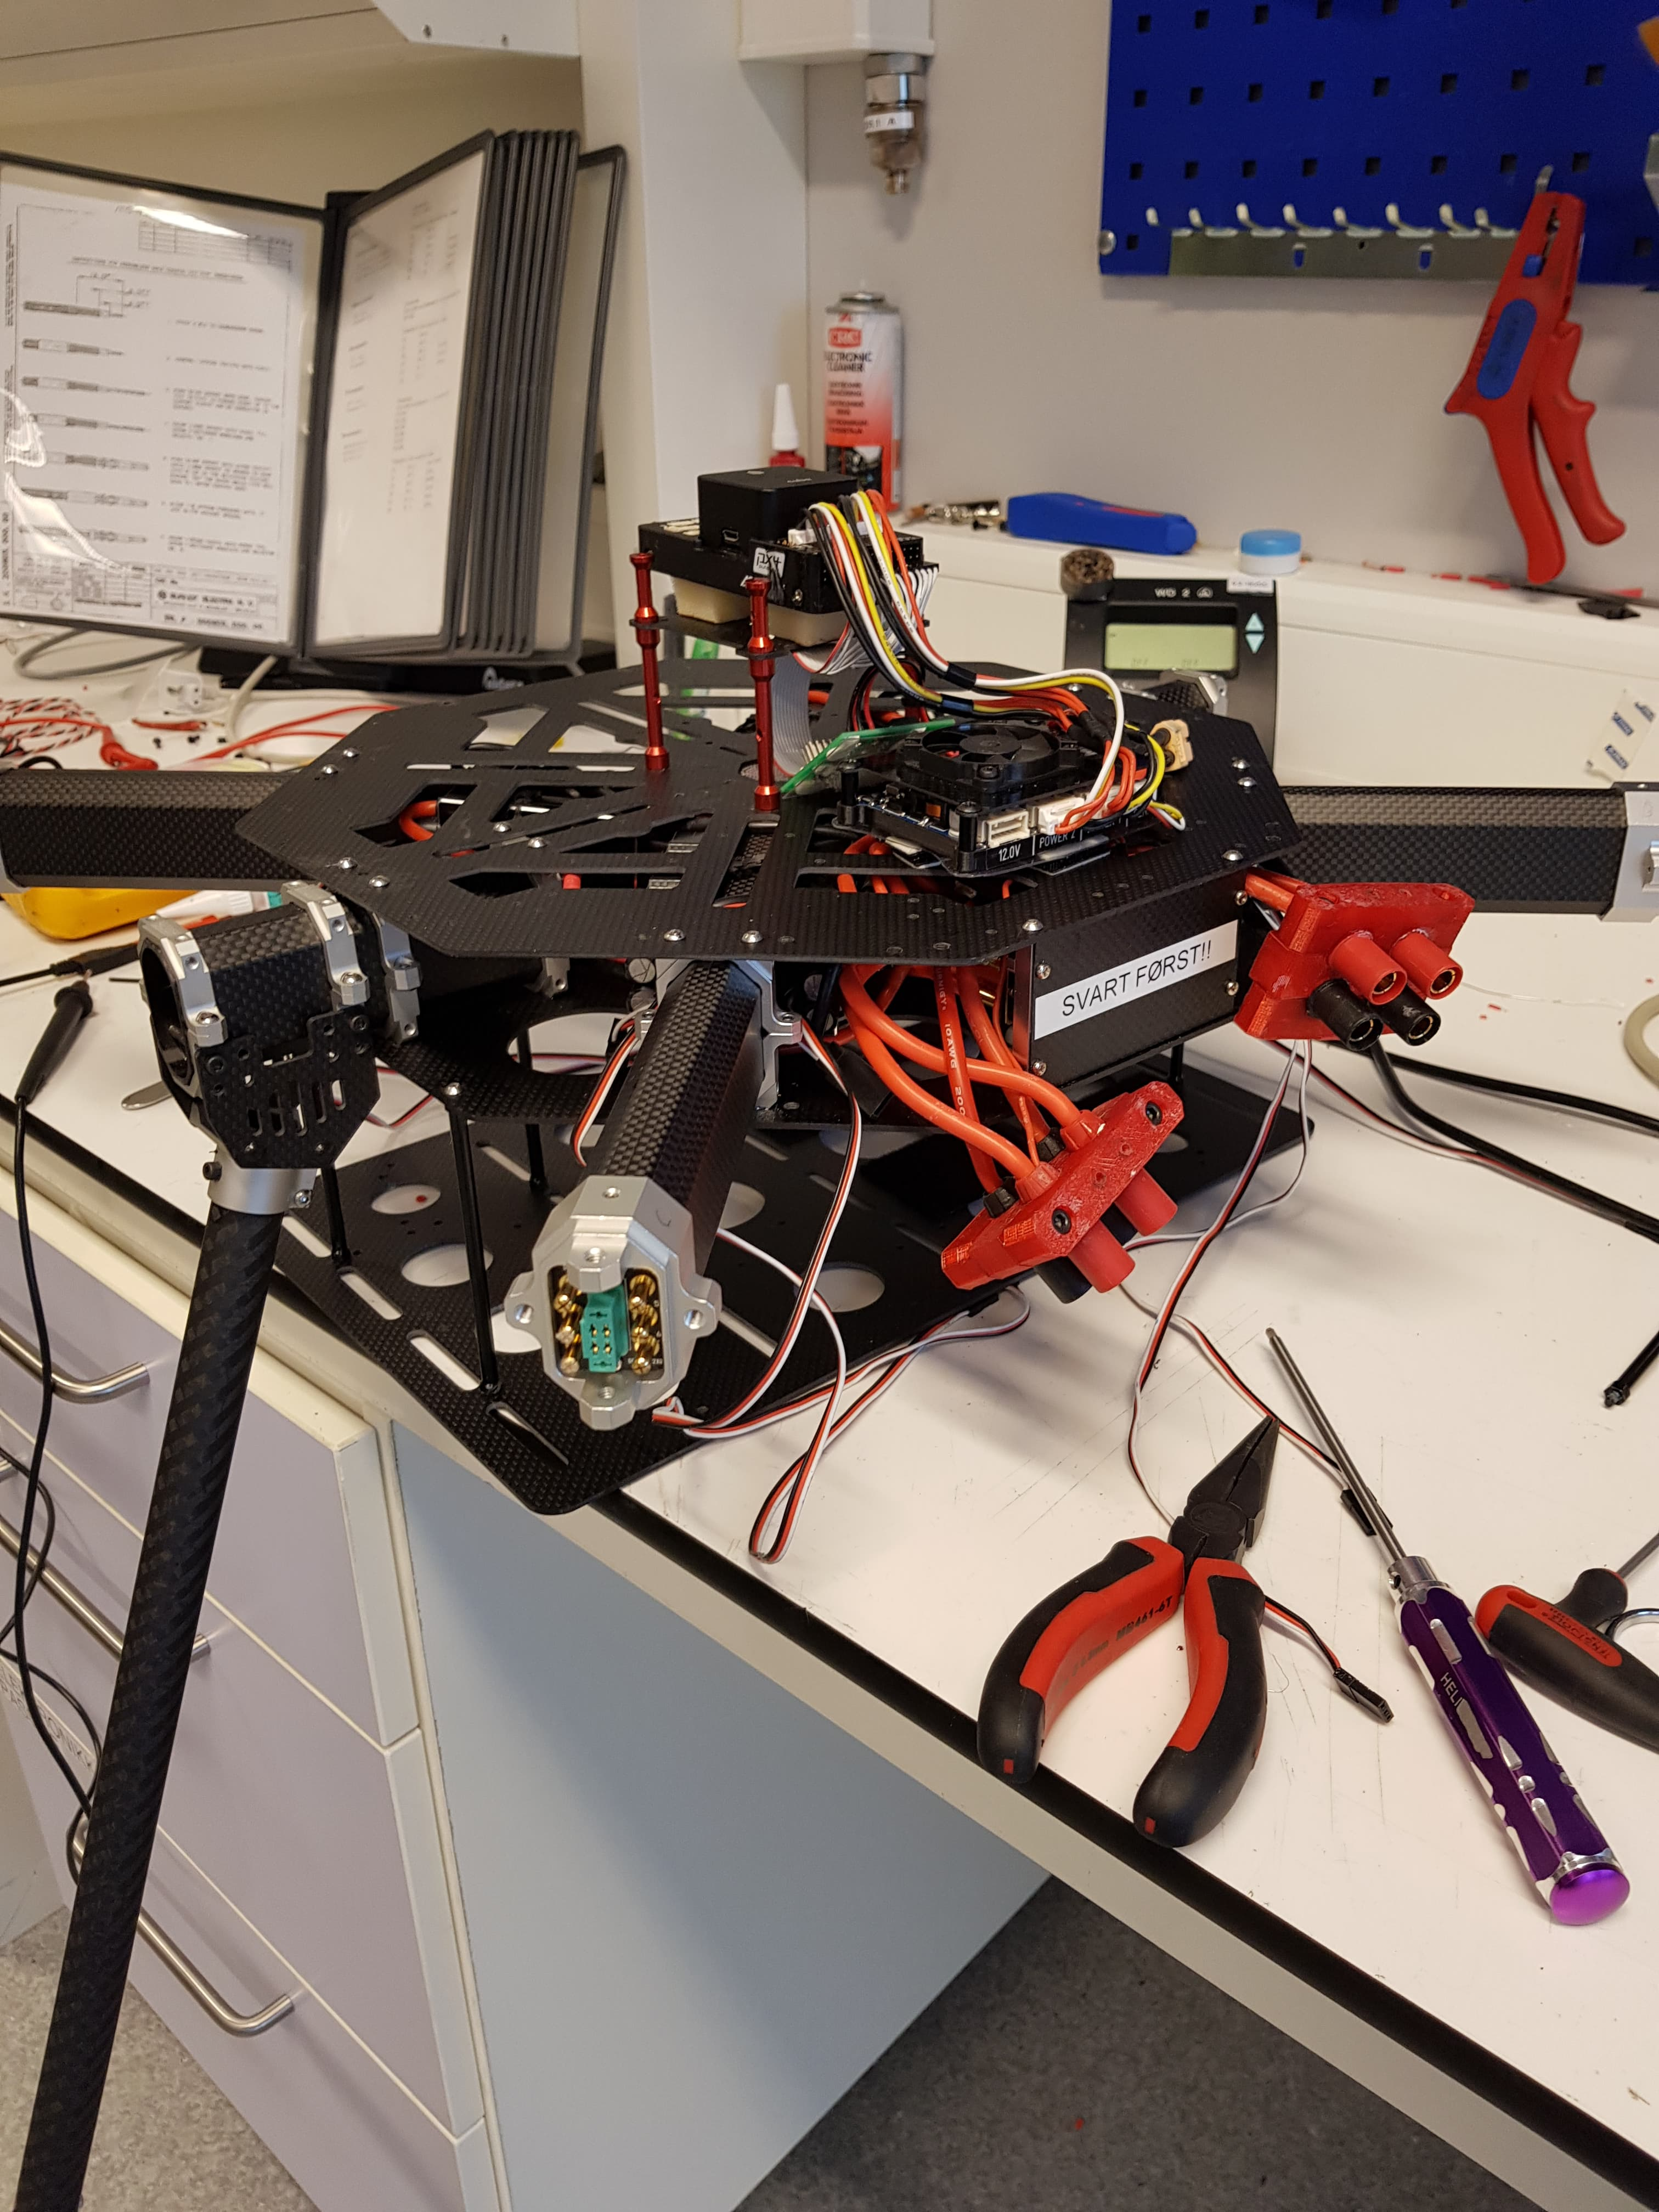
\includegraphics[height = 8cm, width = 0.6\textwidth]{octocopt_x8.jpg}
	\caption{Reparasjonsarbeid på en octocopter i såkalt X8 - konfigurasjon.}
\end{figure}
%Teknisk prosjekt - Cryowing Observer
%\newpage
\begin{figure}[h]
	\centering
	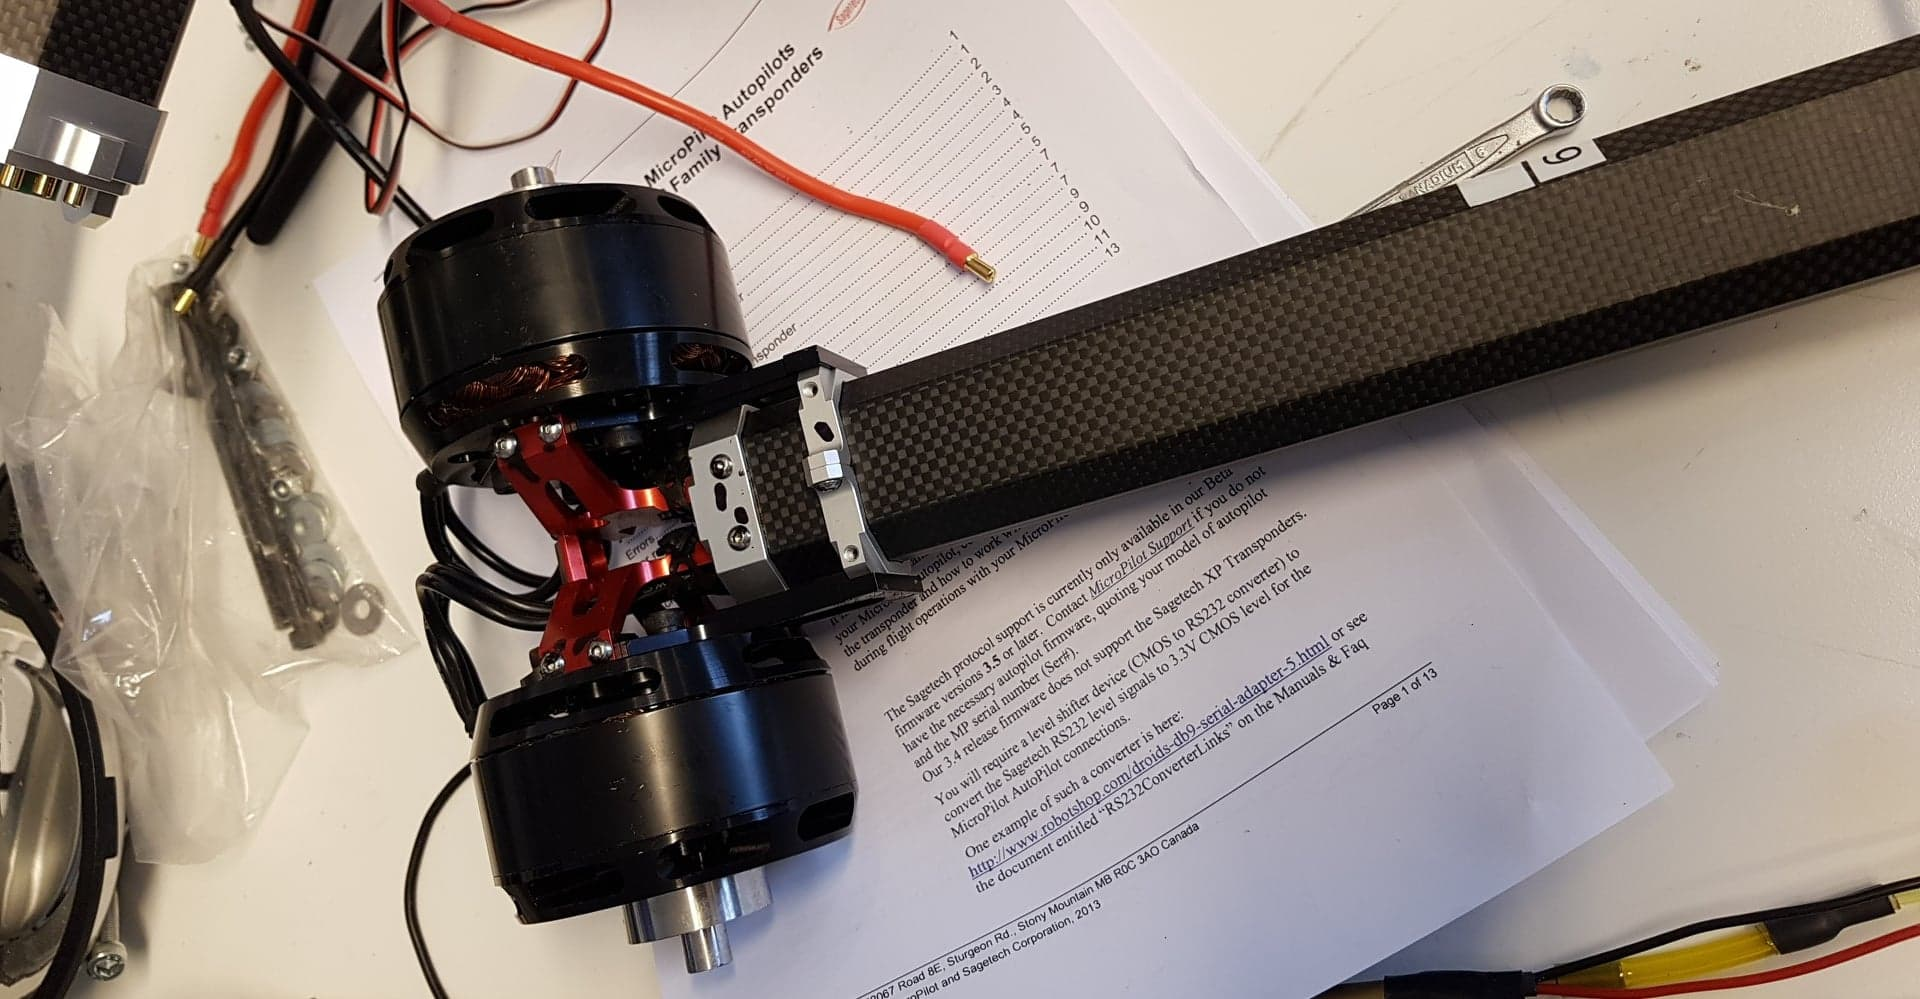
\includegraphics[scale=.2]{octarm_x8.jpg}
	\caption{Montering av nye motorer på ytre armer.}
\end{figure}



\section{Diskusjon \& refleksjon}
\subsection{Lærdom}


\subsection{Konklusjon}



\end{document}